\documentclass[11pt, a4paper]{article}
\usepackage[a4paper, margin=2.5cm]{geometry}
\usepackage{iftex}
\usepackage{graphicx}
\ifPDFTeX
    \usepackage[english]{babel}
\else
    \usepackage{fontspec}
    \usepackage[english, bidi=basic, provide=*]{babel}
    \babelprovide[import, onchar=ids fonts]{english}
    \babelfont{rm}{Noto Sans}
\fi
\usepackage{amsmath}
\usepackage{booktabs}
\usepackage{hyperref}

\hypersetup{
    colorlinks=true,
    linkcolor=blue,
    urlcolor=blue,
    pdftitle={Standard Convolutional Neural Networks on the MAMe Dataset}
}

\newcommand{\pair}[2]{\author{#1 \and #2}}

\title{Deep Learning Lab 1: Standard CNNs on the MAMe Dataset}
\pair{Benjamin ???}{Milan Van den Eede}
\date{\today}

\begin{document}
\maketitle

\section{Experimental Setup and Methodology}

To evaluate the performance of standard Deep Convolutional Neural Networks (CNNs) trained from scratch on fine-grained artwork medium classification, we use the $256 \times 256$ RGB version of the Museum Art Medium (MAMe) dataset. The dataset aggregates 37,407 artworks across 29 medium classes from three major museums and is partitioned into a balanced training set of 20,300 images (700 per class), a balanced validation set of 1,450 images (50 per class), and an unbalanced test set of 15,657 images.

All images are loaded at their native $256 \times 256$ resolution and normalized to the $[0, 1]$ range via pixel rescaling ($1/255$). Training is conducted with a mini-batch size of 128 using categorical cross-entropy loss and the Adam optimizer with an initial learning rate of $\eta = 5 \times 10^{-4}$ and gradient norm clipping ($\text{clipnorm} = 1.0$) to stabilize parameter updates.

Following a systematic three-stage experimental methodology, we progressively explore the bias--variance trade-off across three model configurations:
\begin{enumerate}
    \item \textbf{Underfitting model:} A deliberately low-capacity architecture designed to exhibit high bias and insufficient representational power.
    \item \textbf{Overfitting model:} A deeper, high-capacity architecture trained without regularization or data augmentation to verify that the network can fit the training distribution and to expose its generalization gap.
    \item \textbf{Regularized model:} The same core convolutional backbone refined with data augmentation, weight decay, spatial and standard dropout, adaptive learning rate scheduling, and early stopping to maximize generalization.
\end{enumerate}

\section{Model Architectures}

All three networks follow a sequential encoder--classifier structure built from $3 \times 3$ convolutional layers with \texttt{same} padding and ReLU activations, interleaved with max-pooling layers and terminated by a 29-way softmax output layer. Table~\ref{tab:architectures} summarizes the architectural and training differences between the three configurations.

\begin{table}[htbp]
\centering
\caption{Comparison of the three standard CNN configurations evaluated on the MAMe dataset.}
\label{tab:architectures}
\small
\begin{tabular}{@{}llll@{}}
\toprule
\textbf{Component} & \textbf{Underfit} & \textbf{Overfit} & \textbf{Regularized} \\
\midrule
Conv Blocks (Filters) & 3 (16--32--64) & 4 (32--64--128--256) & 4 (32--64--128--256) \\
Pooling Schedule & $4\times 4, 4\times 4, 4\times 4$ & $2\times 2, 2\times 2, 2\times 2, 4\times 4$ & $2\times 2, 2\times 2, 2\times 2, 4\times 4$ \\
Flattened Feature Dim. & $4\times 4\times 64 = 1{,}024$ & $8\times 8\times 256 = 16{,}384$ & $8\times 8\times 256 = 16{,}384$ \\
Hidden Dense Layer & None & Dense(256, ReLU) & Dense(256, ReLU) \\
Trainable Parameters & 53,309 & 4,590,429 & 4,590,429 \\
Data Augmentation & None & None & Flip, Rot(0.08), Zoom(0.1) \\
L2 Weight Decay & None & None & $10^{-4}$ (Conv \& Dense) \\
Dropout & None & None & Spatial (0.1, 0.2); Dense (0.5, 0.3) \\
LR Schedule / Stopping & Fixed, 30 epochs & Fixed, 30 epochs & ReduceLR + EarlyStop (max 60) \\
\bottomrule
\end{tabular}
\end{table}

\subsection{Underfitting Architecture}
The underfitting model uses only three convolutional blocks (16, 32, and 64 filters), each followed by aggressive $4 \times 4$ max-pooling. This rapidly compresses the spatial dimensions from $256 \times 256$ to $64 \times 64$, $16 \times 16$, and finally $4 \times 4$, discarding fine-grained surface textures (such as brushstrokes, paper grain, and engraving lines) that are critical for distinguishing art media. The flattened 1,024-dimensional vector connects directly to the 29-class softmax layer without an intermediate hidden dense layer, yielding only 53,309 trainable parameters.

\subsection{Overfitting Architecture}
To establish sufficient representational capacity, the overfitting model expands to four convolutional blocks (32, 64, 128, and 256 filters) with gentler $2 \times 2$ pooling in the first three blocks and $4 \times 4$ pooling in the fourth, preserving an $8 \times 8 \times 256$ feature map (16,384 features). These features feed into a fully connected hidden layer of 256 ReLU units before the softmax classifier. In total, the network contains 4,590,429 trainable parameters, of which 4,194,560 (91.4\%) reside in the transition from the flattened feature map to the hidden dense layer. Trained for 30 epochs without regularization or early stopping, this high-capacity classifier head strongly encourages memorization of the training set.

\subsection{Regularized Architecture}
The regularized model retains the exact 4,590,429-parameter backbone of the overfitting model and introduces complementary regularization mechanisms tailored to each part of the network:
\begin{itemize}
    \item \textbf{Online Data Augmentation:} Horizontal flipping (\texttt{RandomFlip}), mild rotations up to $\pm 8\%$ (\texttt{RandomRotation(0.08)}), and random zooming up to $\pm 10\%$ (\texttt{RandomZoom(0.1)}) are applied exclusively during training to increase effective sample diversity while preserving medium-defining textures.
    \item \textbf{L2 Weight Decay:} A penalty of $\lambda = 10^{-4}$ is applied to the kernels of all convolutional layers and the hidden dense layer to discourage overly large weights.
    \item \textbf{Spatial and Standard Dropout:} \texttt{SpatialDropout2D} with rates of 0.1 and 0.2 is placed after Blocks 3 and 4, respectively, dropping entire feature maps to counter spatial correlation in deep activations. Because the dense classifier accounts for over 91\% of all parameters, stronger standard dropout is applied before the hidden dense layer (0.5) and before the output layer (0.3).
    \item \textbf{Adaptive Optimization and Early Stopping:} \texttt{ReduceLROnPlateau} halves the learning rate (down to a minimum of $10^{-6}$) whenever validation loss stagnates for 4 epochs, while \texttt{EarlyStopping} monitors validation accuracy with a patience of 10 epochs ($\text{min\_delta} = 10^{-3}$) and restores the best weights.
\end{itemize}

\section{Learning Curve Analysis}

\subsection{Underfitting Scenario}
As shown in Figure~\ref{fig:underfit}, across the 30 training epochs the underfitting model completely fails to learn discriminative representations for the 29 media. Training accuracy stagnates around 6.5\%--8.0\% (barely above the 3.45\% uniform random baseline), while validation accuracy oscillates erratically between approximately 5.5\% and 10.0\%. Simultaneously, both training and validation cross-entropy loss fail to converge and instead diverge sharply over the course of training. This confirms that the severe spatial downsampling ($4 \times 4$ pooling from the first layer onward) combined with the low parameter budget (53,309 parameters) and lack of a hidden dense layer prevents the network from capturing the complex visual cues required by the MAMe dataset.

\begin{figure}[htbp]
\centering
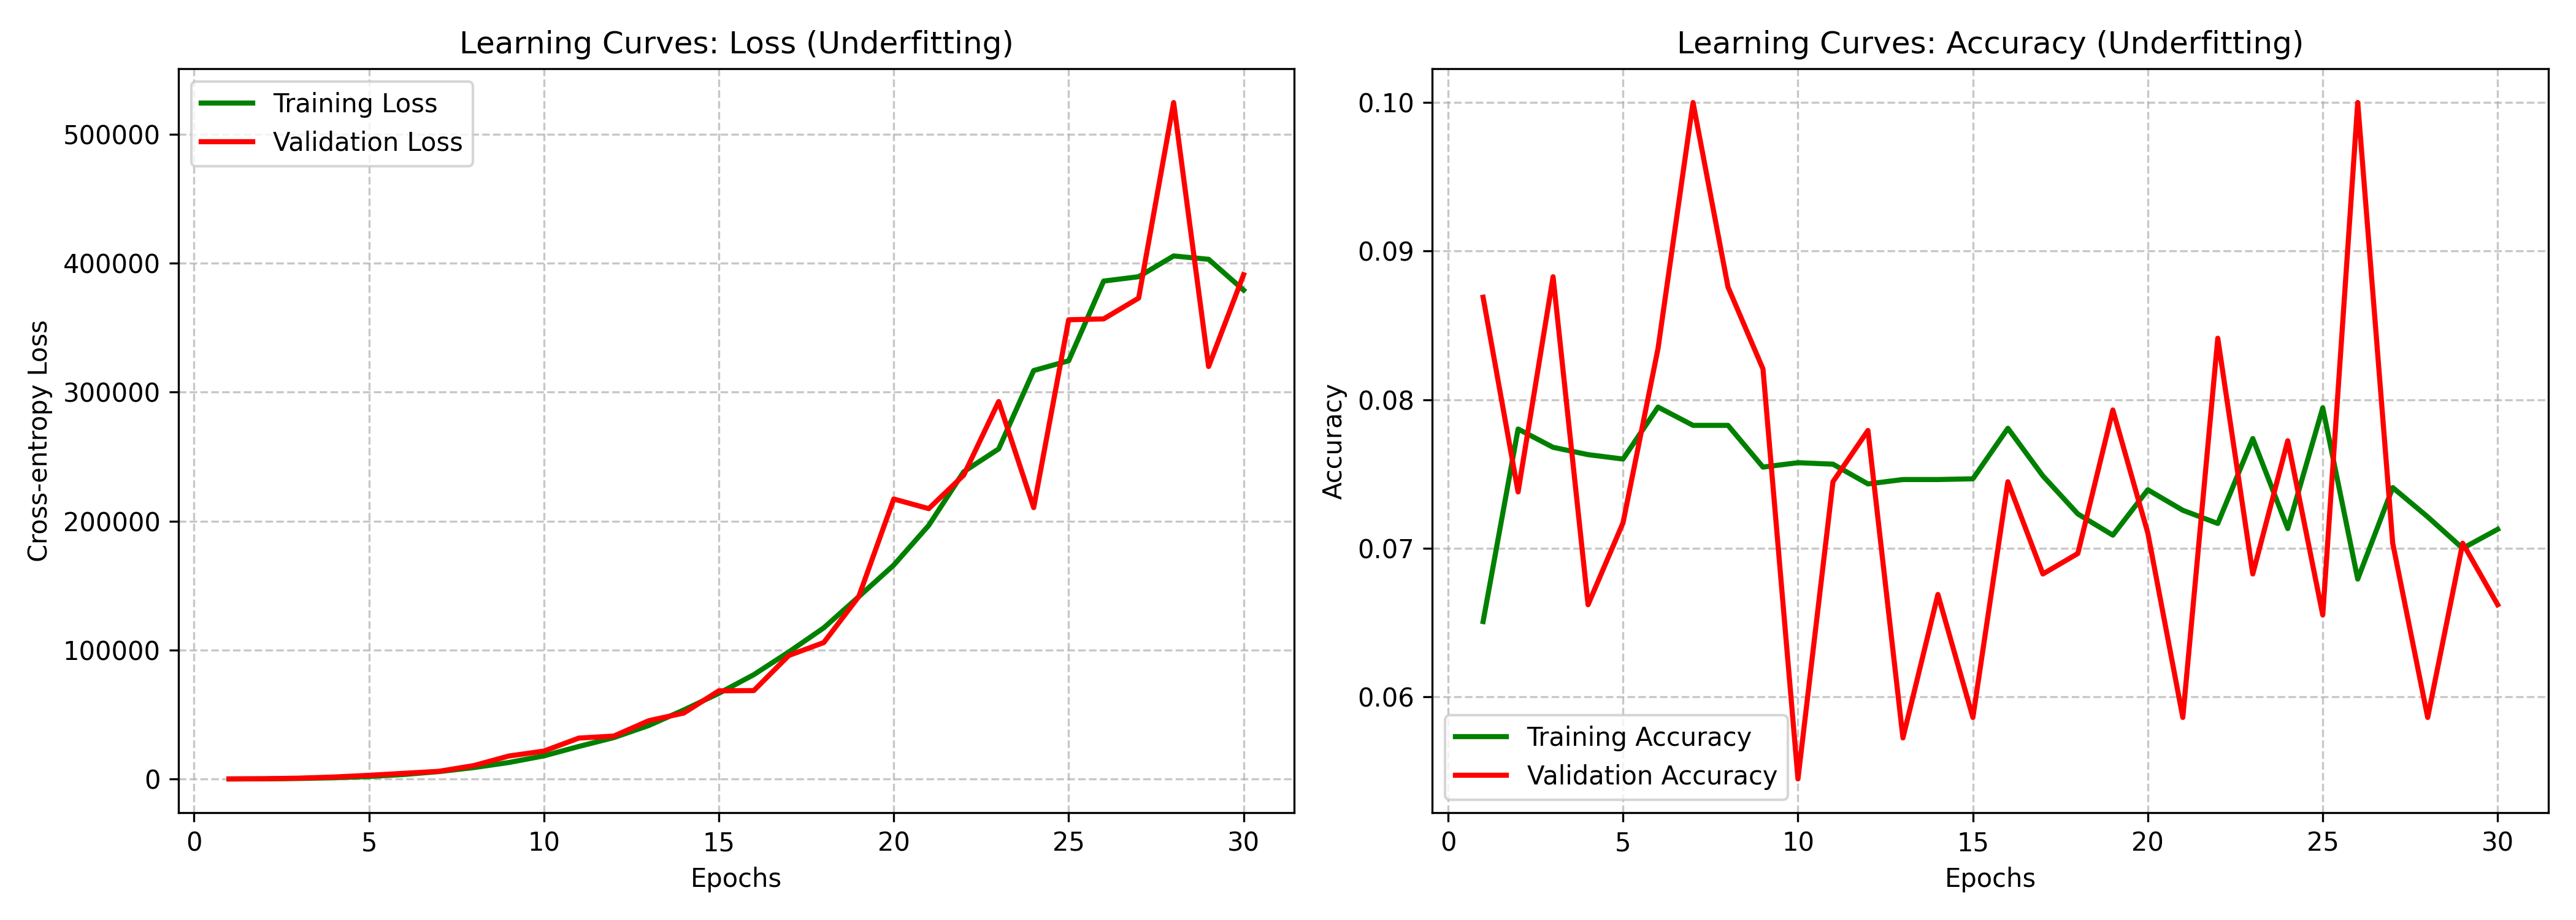
\includegraphics[width=0.95\textwidth]{01_underfit_plot.png}
\caption{Training and validation cross-entropy loss (left) and accuracy (right) for the underfitting model over 30 epochs.}
\label{fig:underfit}
\end{figure}

\subsection{Overfitting Scenario}
Figure~\ref{fig:overfit} illustrates that the unregularized 4-block CNN demonstrates textbook overfitting. Training loss decreases smoothly and monotonically from approximately 2.37 at epoch 1 to nearly 0.04 by epoch 20, while training accuracy climbs rapidly from 30\% to over 93\% by epoch 10 and plateaus at approximately 99\% for the remainder of training. In contrast, validation loss reaches its minimum of roughly 1.12 around epoch 6 and then diverges steadily upward to approximately 2.43--2.58 by epochs 28--30, indicating growing overconfidence on misclassified validation examples. Validation accuracy peaks near 70\% around epoch 16 and then stagnates and declines toward 65.5\% by epoch 30, resulting in a generalization gap of more than 30 percentage points.

\begin{figure}[htbp]
\centering
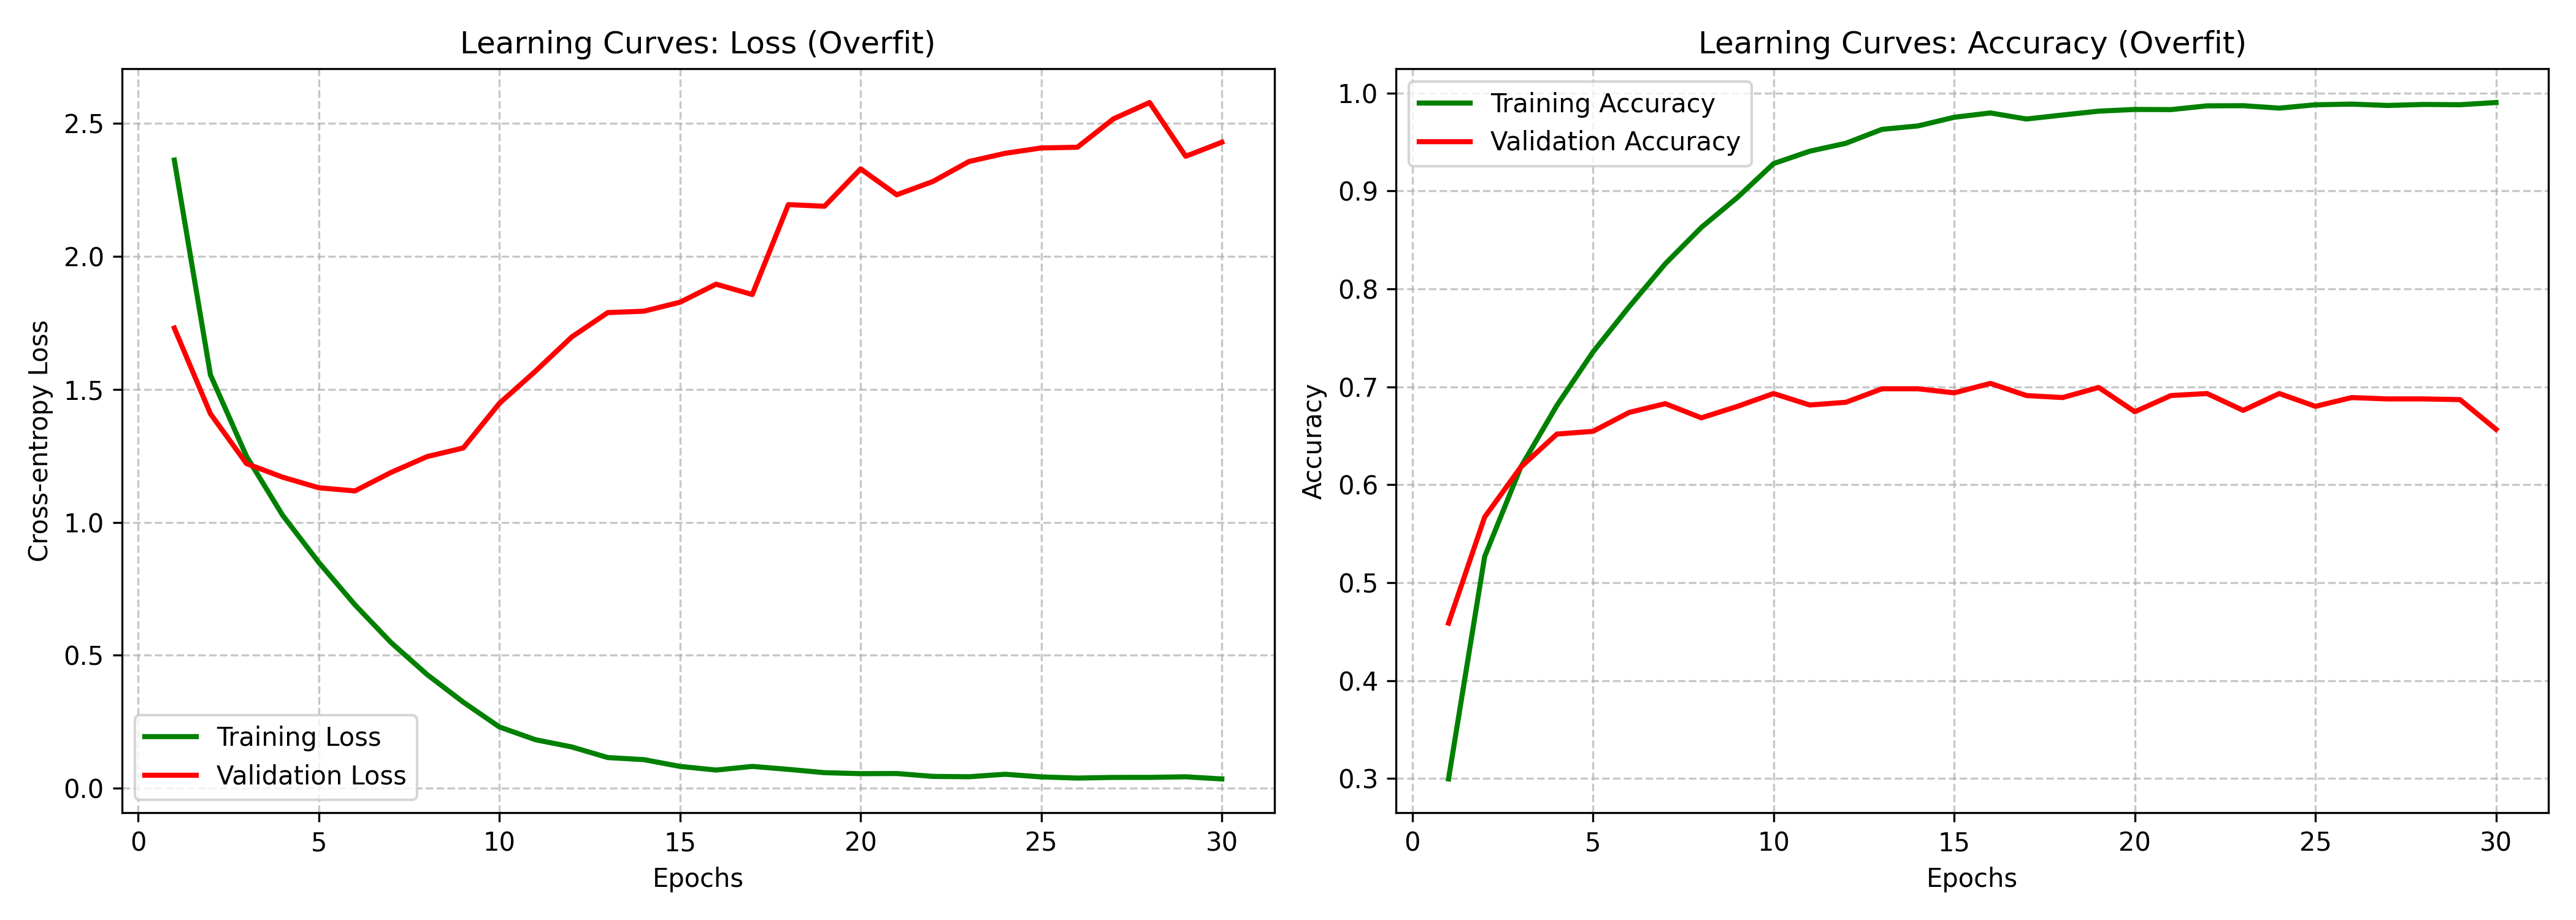
\includegraphics[width=0.95\textwidth]{01_overfit_plot.png}
\caption{Training and validation cross-entropy loss (left) and accuracy (right) for the overfitting model over 30 epochs.}
\label{fig:overfit}
\end{figure}

\subsection{Regularized Scenario}
As depicted in Figure~\ref{fig:regularized}, introducing regularization fundamentally transforms the learning dynamics. During the first 10 epochs, validation loss is slightly lower than training loss (and validation accuracy slightly higher than training accuracy) because data augmentation and dropout are active during training passes but disabled during validation. Both curves progress closely together throughout training, and the catastrophic validation-loss divergence observed in the overfitting model is entirely eliminated. Validation loss decreases from 2.19 at epoch 1 to a minimum of 1.1636 at epoch 26, where validation accuracy reaches its peak of 69.45\%. Because no further validation accuracy improvement exceeds $\text{min\_delta} = 10^{-3}$ over the subsequent 10 epochs, early stopping terminates training at epoch 36 and restores the optimal weights from epoch 26.

\begin{figure}[htbp]
\centering
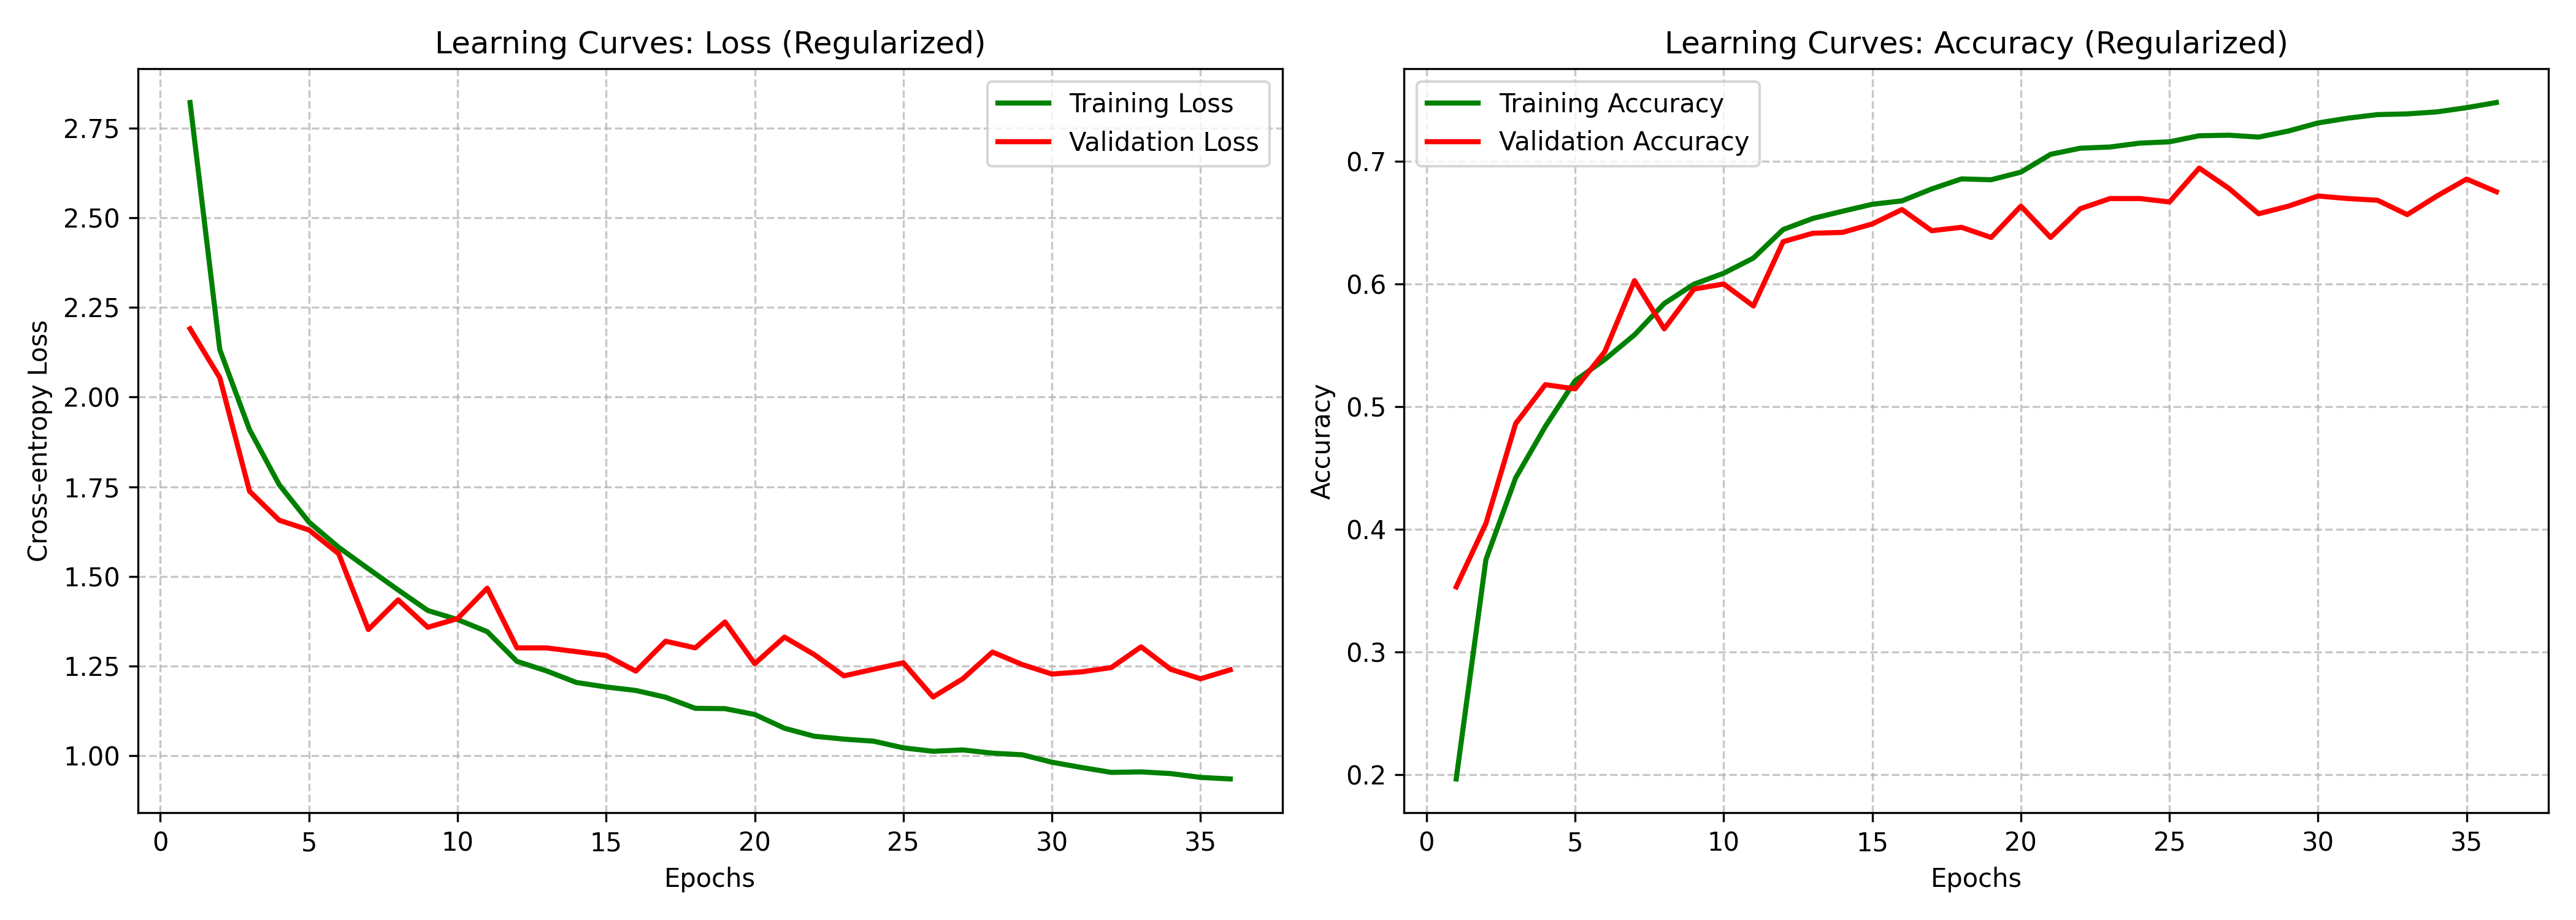
\includegraphics[width=0.95\textwidth]{01_regularized_plot.png}
\caption{Training and validation cross-entropy loss (left) and accuracy (right) for the regularized model (\texttt{01\_regularized\_model}), terminated by early stopping at epoch 36 with best weights restored from epoch 26.}
\label{fig:regularized}
\end{figure}

\section{Final Evaluation}

Because training-time metrics for the regularized model are computed with active dropout and data augmentation, they underestimate the model's true fit on unperturbed training images. To obtain an unbiased assessment of the generalization gap, the restored \texttt{01\_regularized\_model} (epoch 26 weights) was evaluated in pure inference mode across all three dataset splits. The results are summarized in Table~\ref{tab:split_eval}.

\begin{table}[htbp]
\centering
\caption{Inference-mode evaluation of \texttt{01\_regularized\_model} across all MAMe dataset splits.}
\label{tab:split_eval}
\begin{tabular}{@{}lccc@{}}
\toprule
\textbf{Dataset Split} & \textbf{Samples} & \textbf{Loss} & \textbf{Accuracy} \\
\midrule
Train (Inference) & 20,300 & 0.8726 & 77.12\% \\
Validation (Inference) & 1,450 & 1.1636 & 69.45\% \\
Test (Inference) & 15,657 & 1.1990 & 67.53\% \\
\midrule
\textbf{Test Balanced Accuracy (Macro Recall)} & 15,657 & --- & \textbf{68.53\%} \\
\bottomrule
\end{tabular}
\end{table}

In inference mode, the train--validation accuracy gap is reduced to 7.67 percentage points (77.12\% vs.\ 69.45\%), a substantial improvement over the $>30$ percentage-point gap of the unregularized model. Furthermore, the model generalizes robustly to the unseen test set, achieving 67.53\% overall accuracy (loss 1.1990) and 68.53\% balanced accuracy (macro-averaged recall). The small 0.92 percentage-point difference between balanced validation accuracy (69.45\%) and balanced test accuracy (68.53\%) confirms that hyperparameter tuning did not overfit to the validation set.

\section{Summary}

Through a controlled progression from underfitting to overfitting and targeted regularization, our standard 4-block CNN trained from scratch achieves 69.45\% validation accuracy, 67.53\% test accuracy, and 68.53\% test balanced accuracy across 29 artwork media. Combining online data augmentation, L2 weight decay, spatial and standard dropout, adaptive learning rate scheduling, and early stopping effectively eliminates validation-loss divergence and narrows the generalization gap from over 30 percentage points to 7.67 percentage points without modifying the core convolutional backbone.

\end{document}